% Every arrow is an actual map on the stated domain, not an approximate plot.
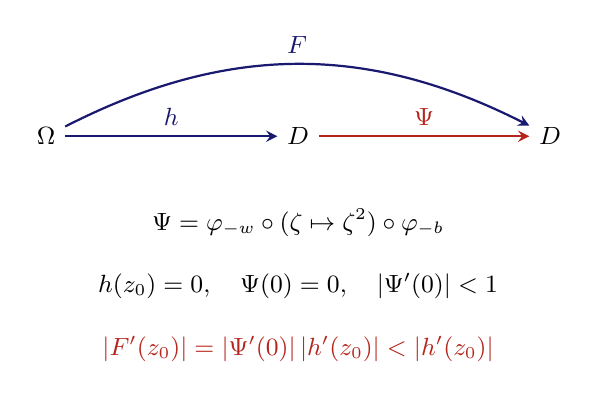
\begin{tikzpicture}[font=\small,>=stealth]
\node (o) at (0,0) {$\Omega$};
\node (h) at (3.2,0) {$D$};
\node (d) at (6.4,0) {$D$};
\draw[->,thick,MidnightBlue] (o)--node[above] {$h$} (h);
\draw[->,thick,BrickRed] (h)--node[above] {$\Psi$} (d);
\draw[->,thick,MidnightBlue] (o) to[bend left=27] node[above] {$F$} (d);
\node[align=center] at (3.2,-1.1) {$\Psi=\varphi_{-w}\circ(\zeta\mapsto\zeta^2)\circ\varphi_{-b}$};
\node[align=center] at (3.2,-1.9) {$h(z_0)=0,\quad\Psi(0)=0,\quad |\Psi'(0)|<1$};
\node[BrickRed,align=center] at (3.2,-2.7) {$|F'(z_0)|=|\Psi'(0)|\,|h'(z_0)|<|h'(z_0)|$};
\end{tikzpicture}
